% !TEX root =  ../report.tex

\section{Research}
\label{s:research}

\subsection{CUDA}
Since this project will require the automatic generation of CUDA from sequential code, it is important to introduce the NVidia hardware, and the C API which will be utilised. The information is pulled from the \textit{NVidia CUDA C Programming Guide} \cite{guide}, which will continue to be used for reference throughout the report.

\subsubsection{Hardware}
GPU hardware is specialised to perform compute-heavy workloads, where the ratio of arithmetic operations to memory operations is high, by devoting more resources to actual data processing. Figure \ref{fig:arch} compares this to a more traditional CPU architecture, which optimises for flow control and data caching:

\begin{figure}[h]
  \centering
  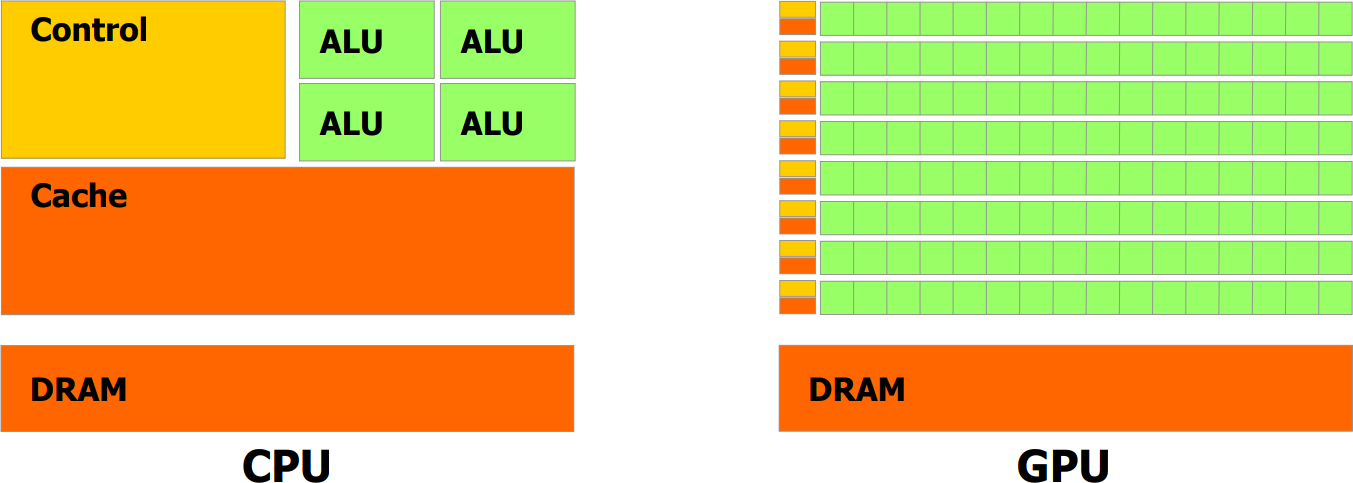
\includegraphics[width=\textwidth]{Architecture}
  \caption{\label{fig:arch} Architecture Comparison. Diagram from \cite[p3]{guide}}
\end{figure}

This structure allows GPUs to excel at performing parallel tasks requiring the same action to be performed on large sets of data, and therefore well suited to the needs of OP2, where a particular function might need to be applied to all edges, or cells, or nodes in the mesh. Since OP2 enforces that the order in which the function is applied to the members of the set must not affect the final result \cite[p4]{manual}, the consideration for data dependencies is largely removed, and operations can be scheduled based on best performance.
\par
Workloads executed on a GPU are divided among a Grid of Blocks, where each Block contains a number of Threads. To allow for simple mapping from the problem to the thread ID, the Block Identifiers, and Thread Identifiers within each block, can be 1D, 2D or 3D \cite[p9]{guide}. Figure \ref{fig:threadgrid} shows an example where 2D identifiers are used.\\
\begin{figure}[h!]
  \centering
  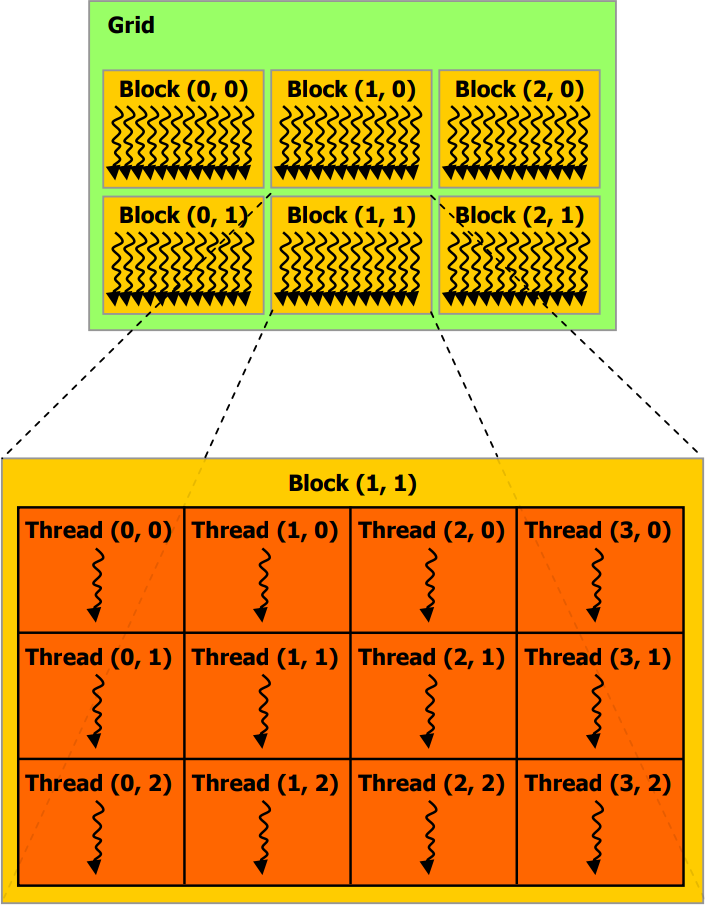
\includegraphics[width=0.5\textwidth]{threadgrid}
  \caption{\label{fig:threadgrid} 2D grid of Blocks and Threads. Diagram from \cite[p9]{guide}}
\end{figure}

\noindent The use of this thread layout will become more clear in the next section, where the invocation of a function to run on a GPU device is described.

\subsubsection{Programming Interface}
The CUDA C API provides two function type quantifiers that will need to be used in the generated code:
\begin{itemize}
\vspace{-.5cm}
\setlength{\itemsep}{0pt}%
\setlength{\parskip}{0pt}%
\item{\verb|__device__|}
\item{\verb|__global__|}
\vspace{-.5cm}
\end{itemize}
Both indicate that the function should be compiled to \textit{PTX}, the CUDA instruction set architecture \cite[p15]{guide}, however the difference is that a function declared \verb|__global__| can be invoked from host (CPU) code,  or device (GPU) code; whereas a \verb|__device__| function can only be called from code already executing on the device \cite[p81]{guide}.
\par
Global functions therefore act as a sort of entry point into device code. They are called using special notation to specify the requested number of blocks and threads per block:
\codeline{function<<< num_blocks, threads_per_block >>>( [arguments...] )}{}
\noindent Where the data type of \verb|num_blocks| and \verb|threads_per_block| can be either of \verb|int| (1D), or \verb|dim3| (1D,2D or 3D) \cite[p9]{guide}. The function body will then be executed $\verb|num_blocks| \times  \verb|threads_per_block|$ times. The Kepler Architecture has an upper limit of 2048 total threads per multiprocessor \cite{kepler}.
\par
Inside the function body, built-in variables can be used to access the thread and block ID of each thread as it executes, and from this determine the work which a certain thread should carry out. Appendix \ref{app:cudaEx} is a CUDA program written during research to build familiarity with the constructs, based on an NVidia tutorial.
\par
In the next section, the OP2 library's exisiting code generation script will be discussed, which can produce code executable on a GPU. This code generator can therefore be use to inform some parts of the new code generation script being produced for this report, to save time that would otherwise need to be spent re-developing solutions that have already been completed.

\subsection{OP2}

\subsubsection{Exisiting Work}

OP2 is an "active library" framework \cite{op2main}, which takes a single application code written using the OP2 Application Programming Interface (API), embedded in either C or Fortran. It uses source-to-source translation to produce multiple solutions, each for different optimised parallel implementations - including CUDA for executing operations on NVidia graphics cards. The generated code is then linked against the OP2 library and compiled to produce an executable for the application, which can run on the desired hardware. It is the extra step of code generation that makes OP2 an "active" library, compared to conventional software libraries.
\par
Since this project is focussed on the GPU back-end, and specifically CUDA for NVidia GPUs, the journal article on the design of OP2 for GPU architectures \cite{gpudesign} is necessary background material, as it covers a lot of important details from the GPU implementation.\\ The paper is summerised in the following section:

\minititle{Designing OP2 for GPU architectures}
This article, originally published in the Journal of Parallel and Distributed Computing in 2013, describes the ey design features of the current OP2 library for generating efficient code targeting GPUs based on NVIDIA’s Fermi architecture. It is worth noting that Fermi is no longer the latest architecture, and the code generation process has been modified since publication, however the article still provides useful information.
\par
One of the key points made in the paper is on the managing of data dependencies (p1454), and the solutions proposed for avoiding errors when incrementing indirectly referenced array, where two edges end up updating the same node. Solutions include an owner of node data which performs the computation; colouring of edges such that no two edges of the same colour update the same node; and atomic operations. In the implementation for this project, atomic operations, which perform read-modify-write operation on one 32-bit or 64-bit word residing in global or shared memory \cite[p96]{guide}, as used to solve this issue.
\par
The paper also introduces the consideration for data layout in memory. Figure \ref{fig:soa_v_aos} demonstrates the different layouts possible when there are multiple components for each element. The paper concludes that the struct-of-arrays layout reduces the total amount data transferred to and from GPU global memory, in some cases by over 50\%.

\begin{figure}[h]
  \centering
  \subfloat[Array of Structs (AOS) layout]
  {
    \begin{tikzpicture}[cell/.style={rectangle,draw=black}, ampersand replacement=\&, space/.style={minimum height=1.5em,matrix of nodes,row sep=-\pgflinewidth,column sep=-\pgflinewidth,column 1/.style={font=\ttfamily}},text depth=0.5ex,text height=2ex,nodes in empty cells]

    \matrix (A) [matrix of nodes, nodes={draw, minimum size=8mm}]{
        0 \& 1 \& 2 \& 3 \& 0 \& 1 \& 2 \& 3 \& 0 \& 1 \& 2 \& 3 \& 0 \& 1 \& 2 \& 3\\};
    \end{tikzpicture}
  }

  \quad

  \subfloat[Struct of Arrays (SOA) layout]
  {
    \begin{tikzpicture}[cell/.style={rectangle,draw=black}, ampersand replacement=\&, space/.style={minimum height=1.5em,matrix of nodes,row sep=-\pgflinewidth,column sep=-\pgflinewidth,column 1/.style={font=\ttfamily}},text depth=0.5ex,text height=2ex,nodes in empty cells]

    \matrix (A) [matrix of nodes, nodes={draw, minimum size=8mm}]{
      0 \& 0 \& 0 \& 0 \& 1 \& 1 \& 1 \& 1 \& 2 \& 2 \& 2 \& 2 \& 3 \& 3 \& 3 \& 3\\};
    \end{tikzpicture}
  }
  \caption{\label{fig:soa_v_aos} Data layouts. Diagram reproduced from \cite{gpudesign}}
\end{figure}

\noindent The SoA layout is enabled by setting the value of an environment variable: \verb|OP AUTO SOA=1| prior to code generation \cite[p13]{manual}.
\par
The existing solution is able to generate optimised CUDA code for a parallel loop; given the set of nodes, edges, cells, or any other collection which it operates over; where the resulting code can assign a set element to a GPU thread where it will be processed by the loop body. It is important to note that the existing implementation for CUDA code generation produces a solution that is compiled entirely ahead of time, i.e. prior to the inputs being known, and therefore is not able to make optimisations based on the mesh input. This project aims to fill this space, and determine if there is benefit to be gained from such optimisations.

\subsubsection{OP2 Applications}
There are a number of industrial applications that have been implemented using OP2, which would immediately benefit from any optimisation of generated code, including Airfoil \cite{airfoil} - a non-linear 2D inviscid airfoil code; Hydra \cite{hydra} - Rolls Royce’s turbomachinery simulator, and Volna \cite{volna} - a finite-volume nonlinear shallow-water equation solver used to simulate tsunamis.
\par
They make use of the abstraction provided by OP2, allowing scientists and engineers to focus on the description of the problem, and seperates the consideration for parallelism and data-movements into the OP2 library and code generation.
\par
A further benefit is that such applications could be ported onto a new generation of hardware which might be developed in the future, with only the OP2 backend library needing to be modified to support the new hardware instead of every application individually. This portability can save both time and money in development if multiple different hardware platforms are desired to be used.
\par
Later in this report we will see Airfoil used as a benchmark, to determine whether the new optimisation presented in the report is likely to provide benefit to other OP2 applications.

\subsection{Related Work}

\subsubsection{Similar Libraries}

\subsubsection{JIT}
\label{sec:rw_JIT}
